\documentclass{article}
\usepackage{epsfig}
\usepackage{graphicx}
\usepackage[top=0.50in, bottom=0.50in, left=0.65in, right=0.75in]{geometry}
%\usepackage[a4paper, total={6in, 10in}]{geometry}
\usepackage[table]{xcolor}
\usepackage{tikz}
\usepackage{algorithm}
\usepackage{mathtools}
\usepackage{amsmath,amssymb}
\usepackage[]{algpseudocode}
\usepackage{enumitem}
\title{CS345 Theoretical Assignment 4 \\ }
\author{\vspace{2mm} \large Ayush Agarwal, 13180 \\ M.Arunothia, 13378}
\date{}
\begin{document}
\maketitle
\tableofcontents
\newpage
\section{Any Guarantee of our First-Attempt Algorithm}
\subsection{Counter Example}
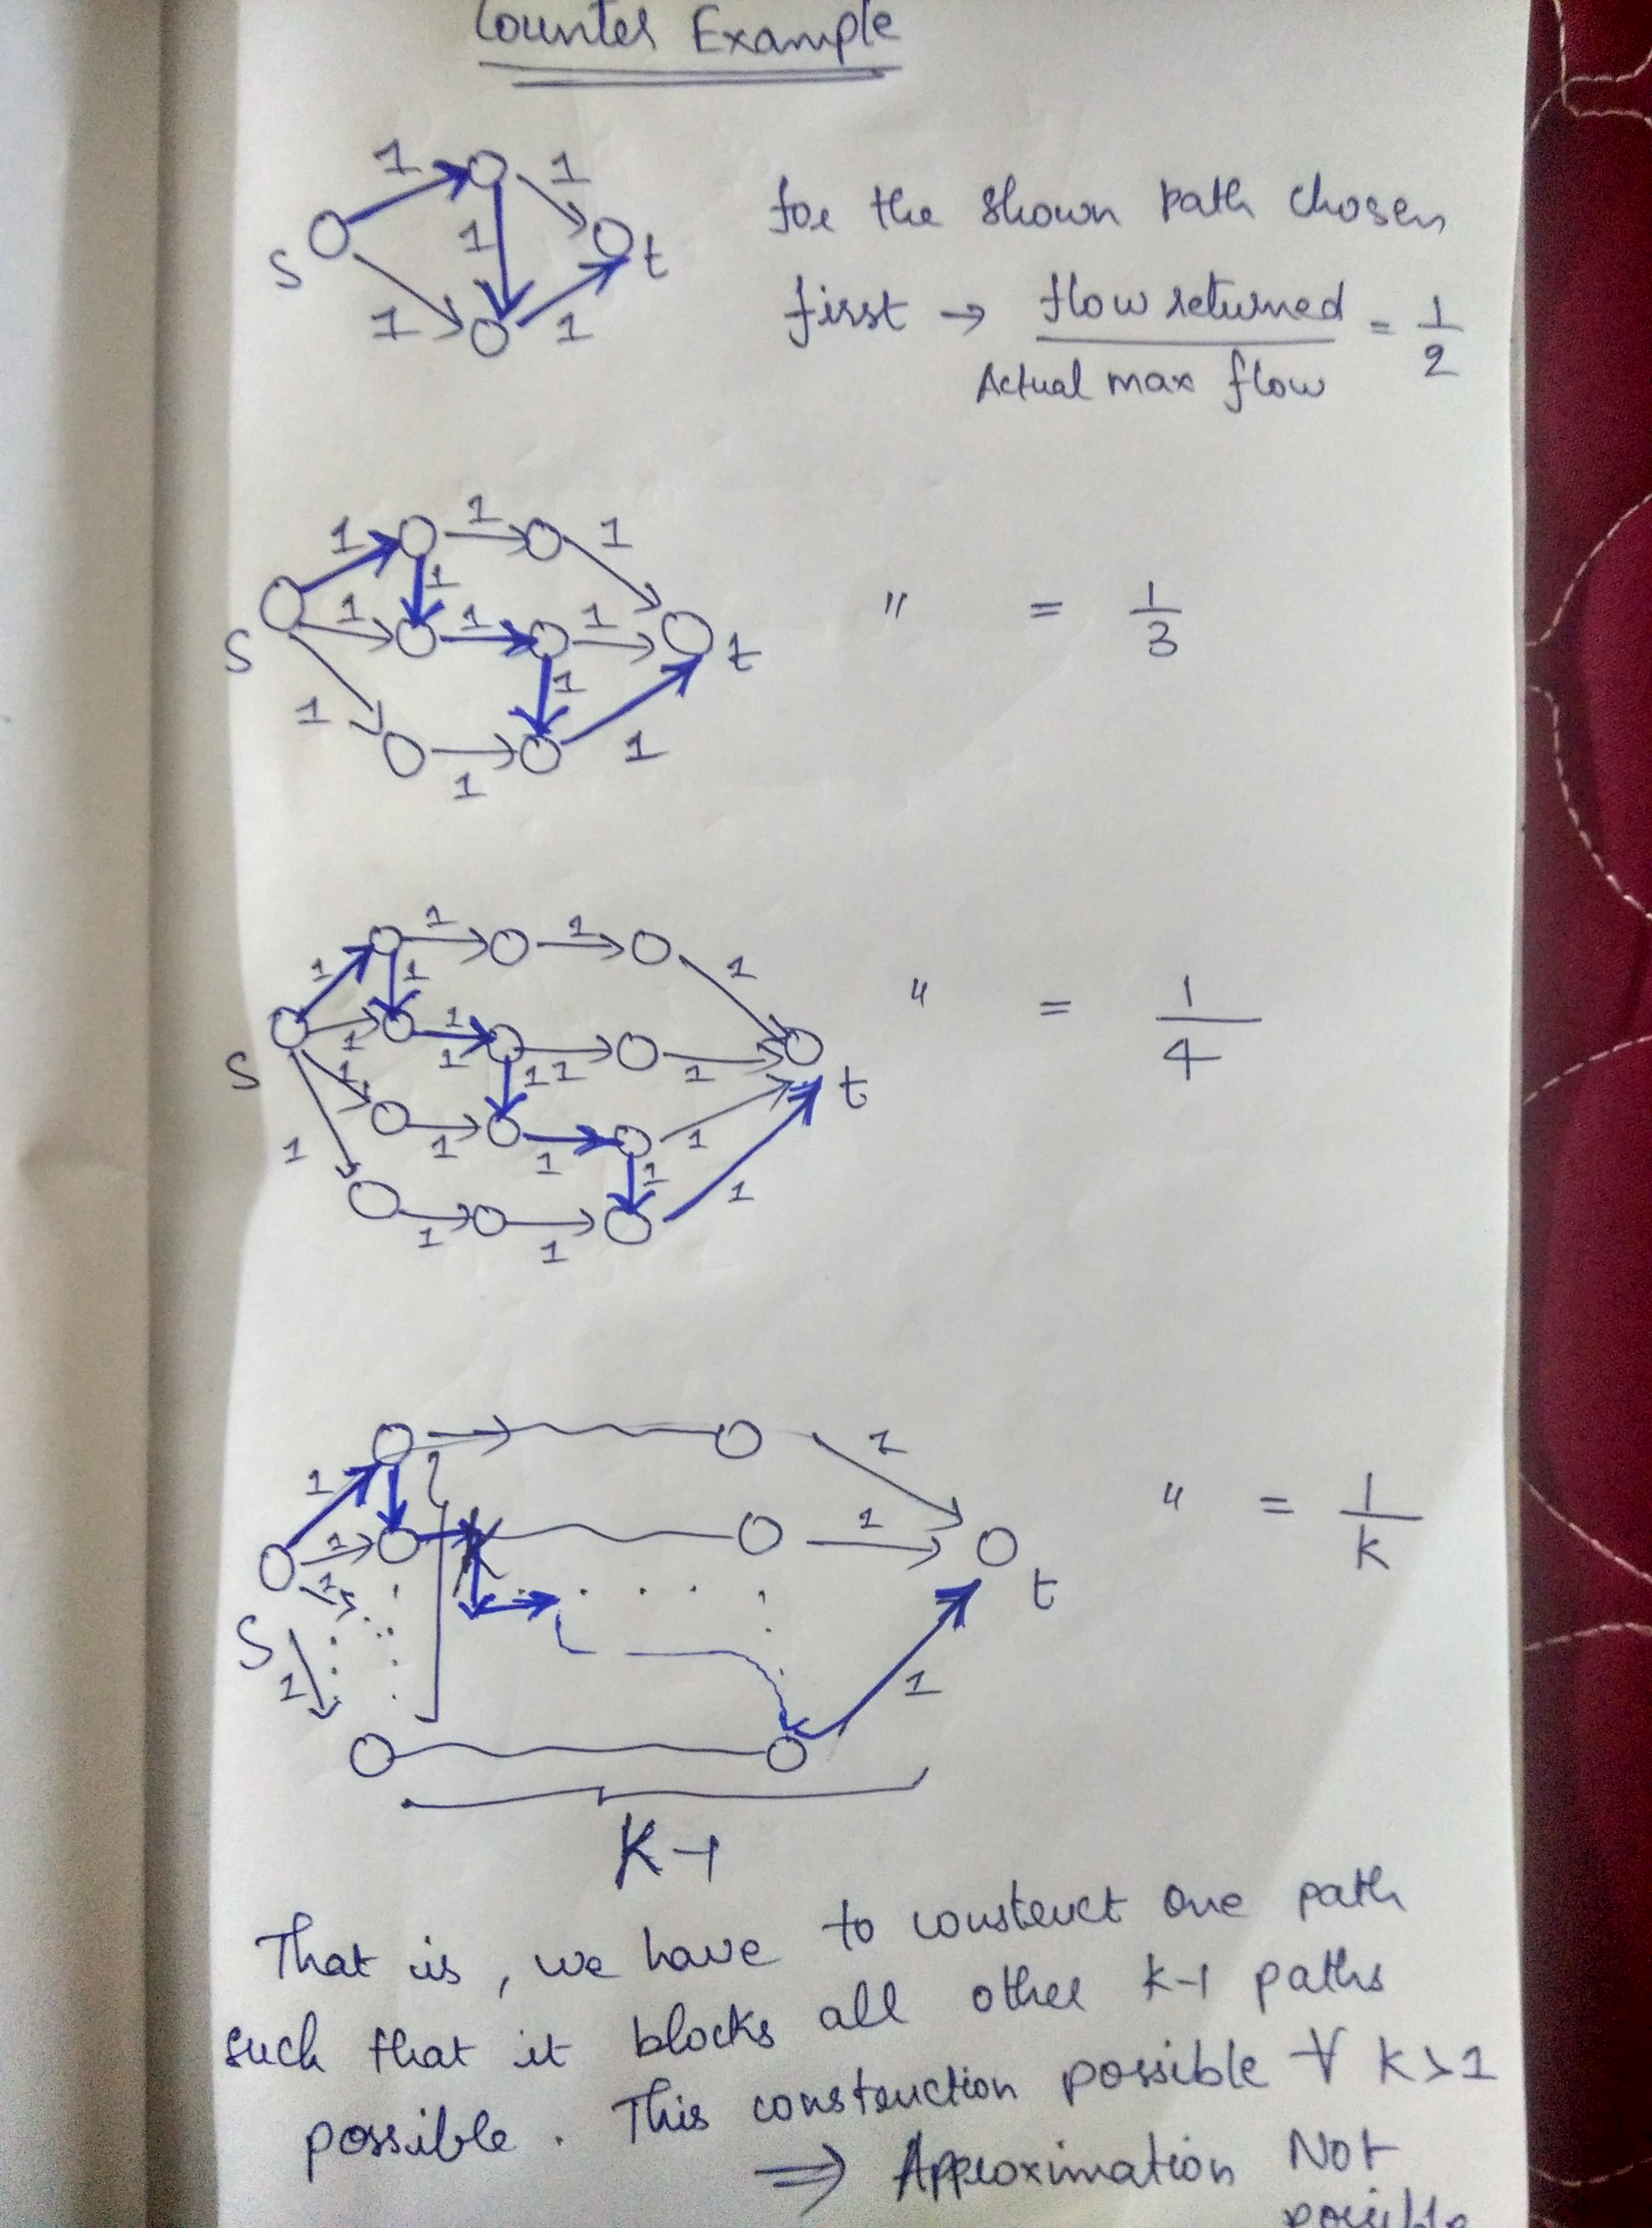
\includegraphics[scale=0.5]{1.jpg}
\newpage
\section{A max flow application}
\subsection{Without Extra Constraint}
\subsubsection{Overview}
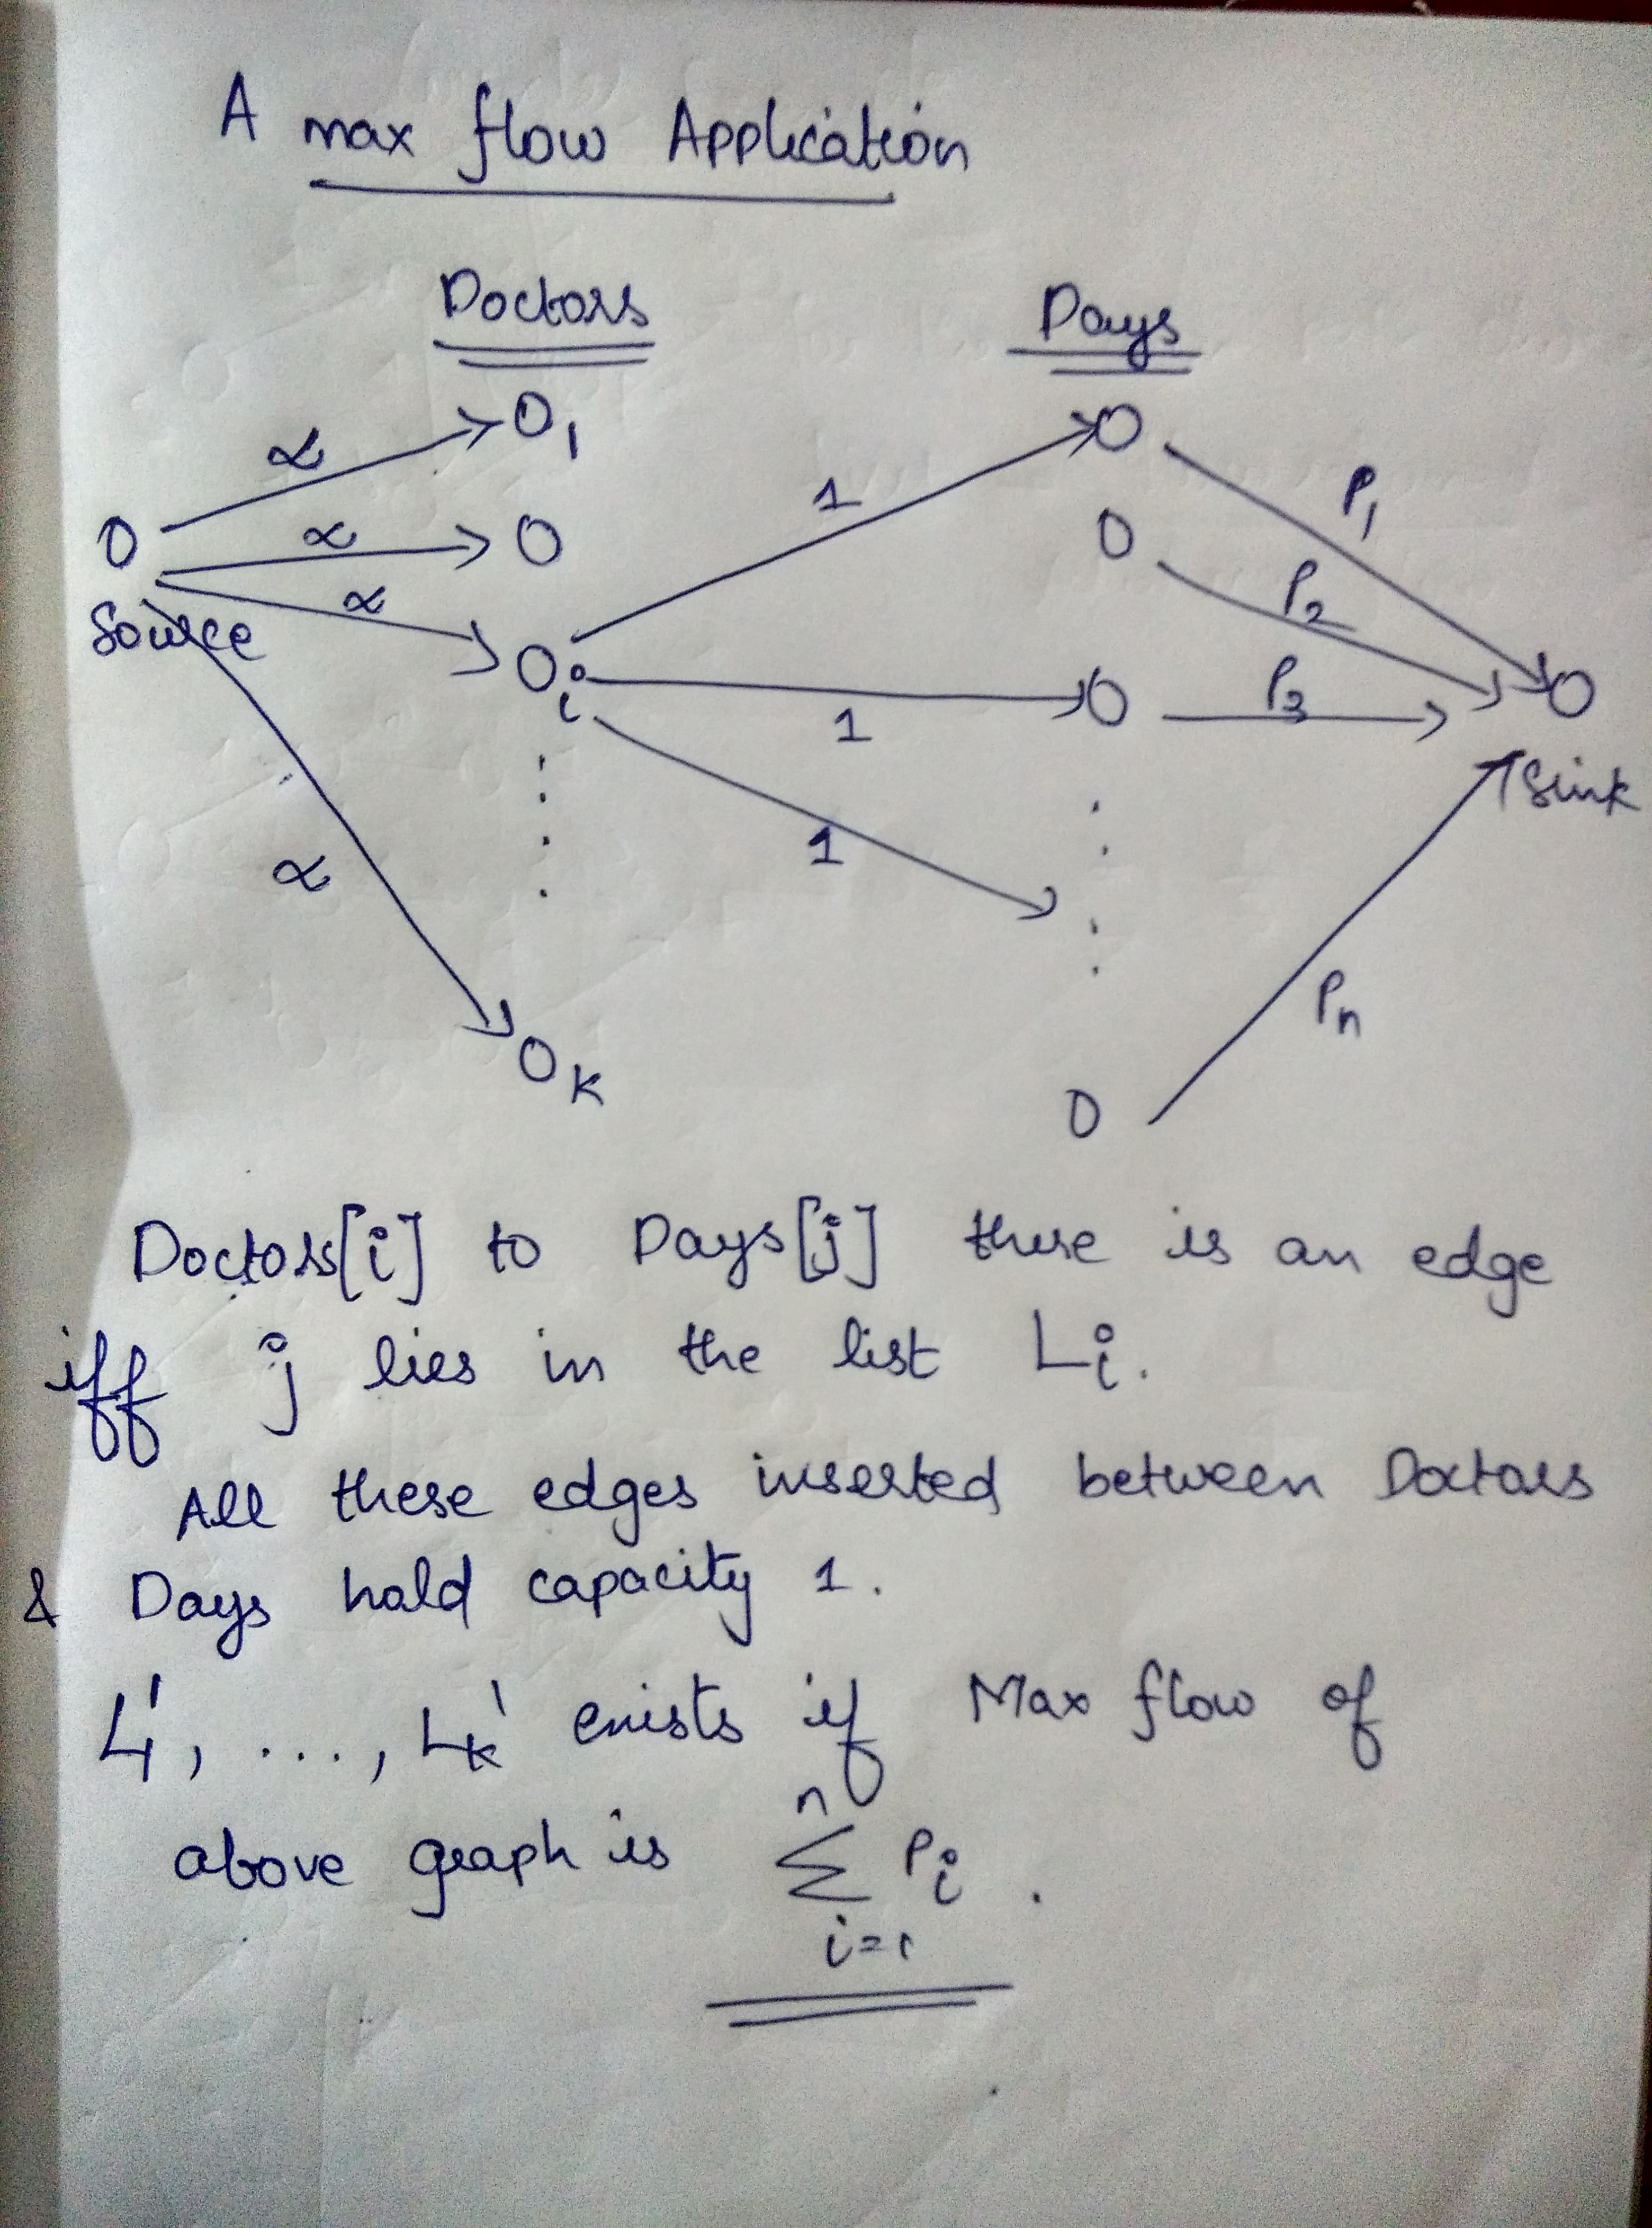
\includegraphics[scale=0.15]{3a.jpg}
\subsubsection{Notations}
$p_i$ denotes the exact number of doctors required on day $i$ \\
$L_i$ denotes the list of days where doctor $i$ is available \\
$L'_i$ denotes the list of days that doctor $i$ has to work to produce the required match. Note, $L'_i \subseteq L_i$\\
$D = \sum_{i=1}^{n} p_i$ \\
$n$ = Number of days in total \\
$k$ = Number of Doctors in total \\ 
\subsubsection{Claim}
Construction of $L'_i$s is possible if and only if the max-flow in the s-t graph is D.
\subsubsection{Proof}
\newpage
\subsection{With Extra Constraint}
\subsubsection{Overview}
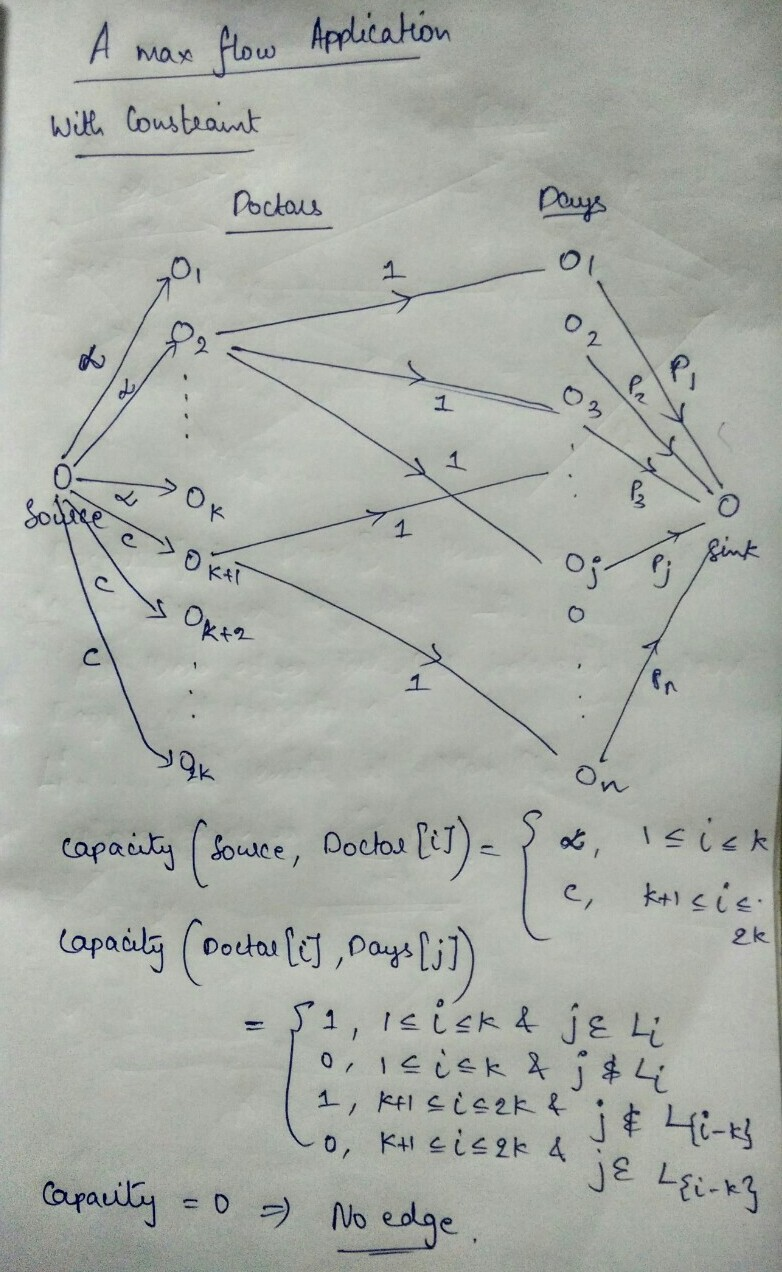
\includegraphics[scale=0.5]{3b.jpg}
\subsubsection{Claim}
\subsubsection{Proof}
\end{document}